% Chapter Template

\chapter{Approach and direct formulation of noise analysis} % Main chapter title

\label{approach} % Change X to a consecutive number; for referencing this chapter elsewhere, use \ref{ChapterX}

\lhead{\emph{Approach and direct formulation of noise analysis}} % Change X to a consecutive number; this is for the header on each page - perhaps a shortened title

%----------------------------------------------------------------------------------------
%	SECTION
%----------------------------------------------------------------------------------------
\section{Direct formulation of noise analysis} \label{direct_approach}
The intention behind this study is to perform a flow field noise analysis in CFD without implementation of acoustical analogies to the CFD code itself. Moreover, very limited information on direct formulation of noise analysis was found during the research, with even fewer research on acoustical near field of transonic axial compressors or axial fans of twin spool jet engines.

The process for the direct formulation noise analysis is following:
\begin{enumerate}
\item Obtain raw flow field data of static pressure, velocity magnitude from CFD analysis.
\item Perform averaging over time of pressure and velocity magnitude for each point or cell in the flow field (equation \ref{eq:avg}).
\item Obtain offset from mean static pressure and velocity magnitude for every timestep for every point/cell in the saved flow field (equation \ref{eq:off}).		
\end{enumerate}

%The process purposely omits transformation of pressure to complex form and forces the analysis on direct signal as measured by a pressure sensor.

\begin{equation} \label{eq:avg}
\bar{p} = \frac{1}{n} \sum_{i=1}^{n} p_i \qquad and \qquad \bar{u} = \frac{1}{n} \sum_{i=1}^{n} u_i
\end{equation}

\begin{equation} \label{eq:off}
p_{i \; sound} = p_i - \bar{p} \qquad and \qquad u_{particle} = u_i - \bar{u}
\end{equation}

Sound pressure signal and flow velocity offset is obtained for every node or cell centroid throughout the simulation flowtime. This dataset can be now post processed 
Dataset obtained in described manner now contains sound pressure of the flow field in every mesh node or cell centroid throughout the computational time. The dataset is now post processed to obtain quantity information of the acoustic nearfield. 

RMS sound pressure level can be obtained from the sound pressure data with use of the formula \ref{eq:RMSp}.

\begin{equation} \label{eq:RMSp}
p_{rms} = \sqrt{\frac{\sum_{i=1}^{n} p_{i \; sound}^{2}}{n}}
\end{equation}

Sound pressure decibel level (SPLdB) is compuded using formula \ref{eq:SPLdB} with standard reference pressure $p_{ref} = 0.00002 Pa$.

\begin{equation} \label{eq:SPLdB}
SPLdB = 20 \cdot \log_{10}\left(\frac{|p_{i \; sound}|}{p_{ref}}\right)
\end{equation}



%Such information may be now post processed for average Root Mean Square of acoustic pressure \& noise intensity and other appropriate figures used in noise analysis including Fourier analysis.

%Proposed method and code developed for this purpose will work on compressible transient CFD analysis returning pressure flow field as a result. Therefore it is required to perform a CFD analysis that will contain pressure flow field to be interpreted as sound. To accomplish that, there are some requirements towards mesh sizing, time stepping information and obtaining the flow field solution.

%-----------------------------------
%	SECTION
%-----------------------------------
\section{CFD analysis requirements} \label{cfdreq}
References \citep{Light1}, \citep{Light2}, \citep{FWH} and \citep{curle} provide a theoretical insight on generating sound in fluid flow due to shear mixing of flows or by implementing a solid boundary in the flow. General remark is: any source of turbulence that result in pressure fluctuation will result in generating sound. Therefore the main requirement for used CFD code for direct noise analysis is the capability of resolving turbulent flow and corresponding fluctuations of the pressure and density.

This approach requires using a finite volume method (fvm) CFD analysis.

%Morbi rutrum odio eget arcu adipiscing sodales. Aenean et purus a est pulvinar pellentesque. Cras in elit neque, quis varius elit. Phasellus fringilla, nibh eu tempus venenatis, dolor elit posuere quam, quis adipiscing urna leo nec orci. Sed nec nulla auctor odio aliquet consequat. Ut nec nulla in ante ullamcorper aliquam at sed dolor. Phasellus fermentum magna in augue gravida cursus. Cras sed pretium lorem. Pellentesque eget ornare odio. Proin accumsan, massa viverra cursus pharetra, ipsum nisi lobortis velit, a malesuada dolor lorem eu neque.


%-----------------------------------
%	SECTION
%-----------------------------------
\section{Mesh sizing requirements} \label{meshsize}
Let's assume a sinusoidal pressure fluctuation $y(t)$ (equation \ref{eq:sine} of ordinary frequency of $f$ and amplitude $A$ moving through ambient medium, for more than 5 cycles at speed of sound \ref{eq:sos}. The mathematical and numerical methods for solving flow field described in section above are capable of computing such pressure fluctuation in a fine resolution mesh. 

\begin{equation} \label{eq:sine}
y(t) = A sin(2 \pi f t + \phi)
\end{equation}

\begin{equation} \label{eq:sos}
a = \sqrt{\kappa R T}
\end{equation}

Both cell size and time step size are limited by the wave length, and therefore frequency of the discussed pressure fluctuation. The wavelength is calculated by formula \ref{eq:wl}.

\begin{equation} \label{eq:wl}
\lambda = \frac{v}{f}
\end{equation}

Considered fluctuation travels through the finite volumes in the stationary CFD mesh. Pressure value is measured at the cell center for each timestep. At this stage, it is assumed that timestep is "good enough" for the analysis. Four possibilities are to be discussed 

%\begin{itemize}
\textbf{Scenario 1:} wavelength is smaller than the edge length of the cell in the direction of propagation. In this condition, the pressure fluctuation performs a number of cycles within one cell (Fig. \ref{scen1}). Due to the numerical approach, such fluctuation will not be computed and recorded by data acquisition at the cell centroid or at node coordinates.

\begin{figure}[h!]
\centering % bo \centering nie wstawia dodatkowego odstępu
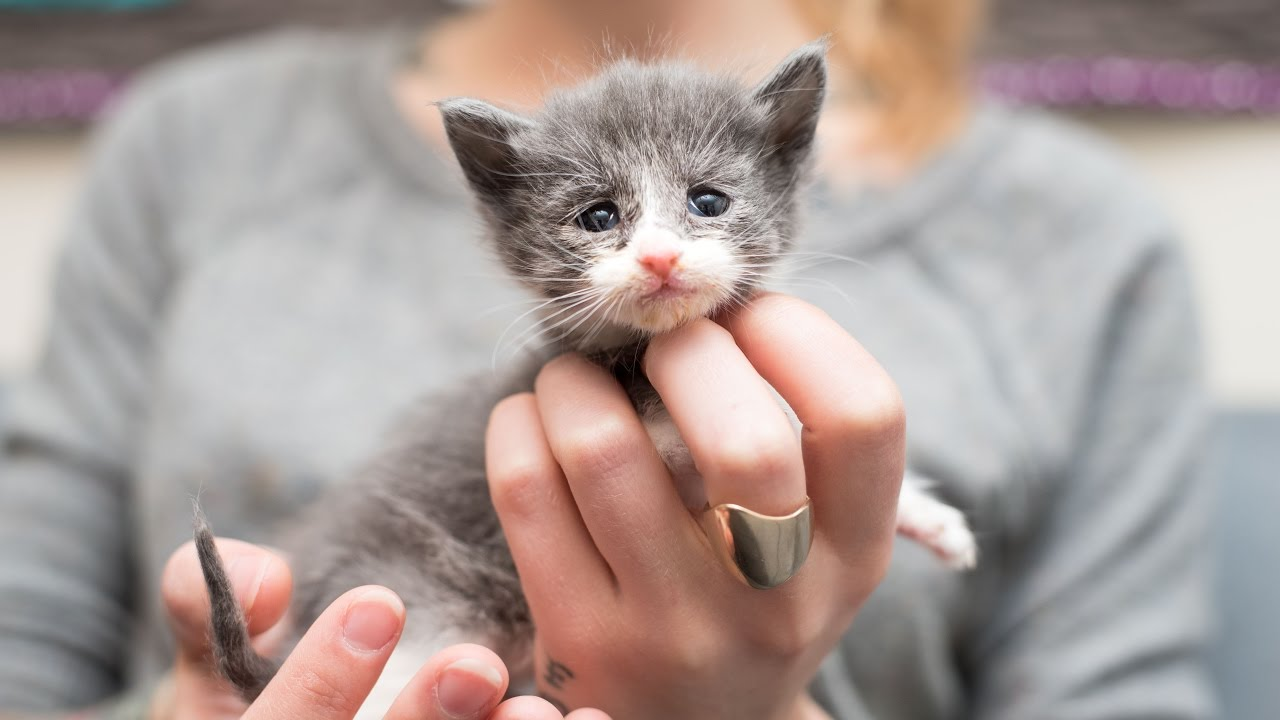
\includegraphics[width=0.5\textwidth]{Pictures/kitten-placeholder.jpg}
\caption{Scenario 1. Wavelength smaller than cell edge length}
\label{scen1}
\end{figure}

\textbf{Scenario 2:} wavelength and cell edge length in the direction of propagation are equal. In this condition, the pressure fluctuation performs one cycle within one cell in the direction of the fluctuation propagation (Fig. \ref{scen2}). Such pressure change will be also filtered out by the numerical scheme.

\begin{figure}[h!]
\centering % bo \centering nie wstawia dodatkowego odstępu
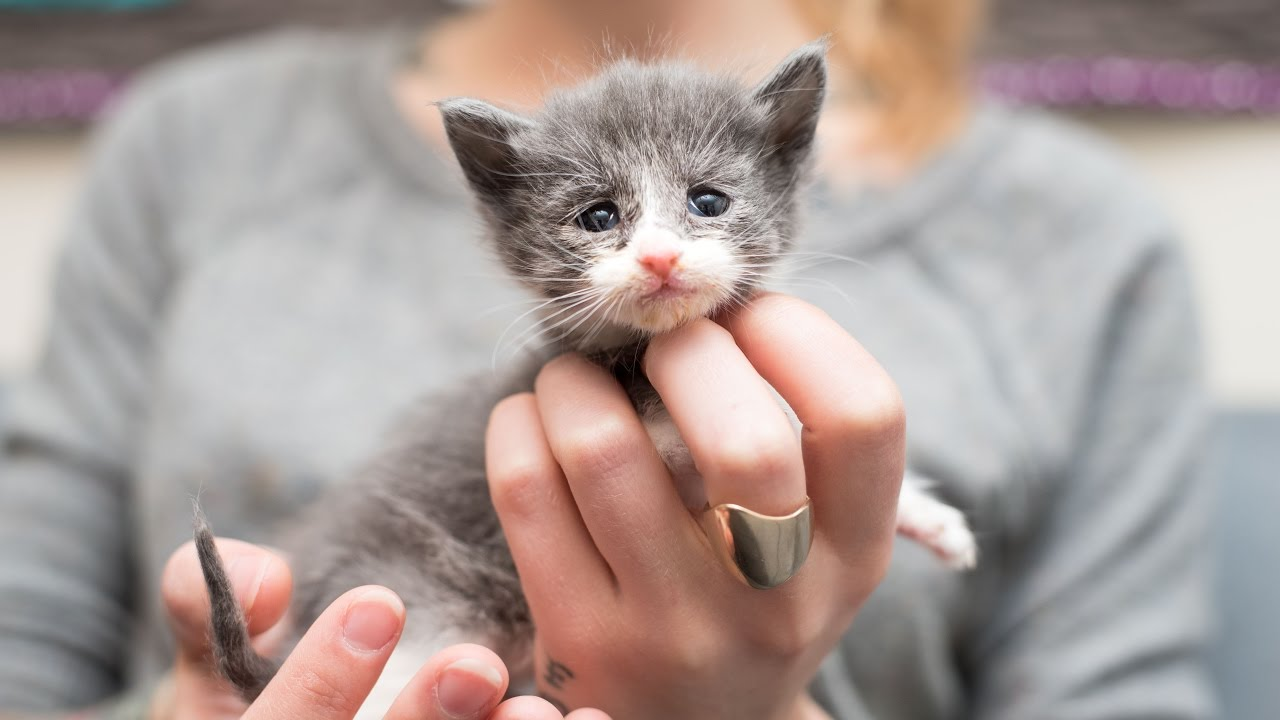
\includegraphics[width=0.5\textwidth]{Pictures/kitten-placeholder.jpg}
\caption{Scenario 2. Wavelength equal to cell edge length}
\label{scen2}
\end{figure}

\textbf{Scenario 3:} wavelength is equal to 4 minimum cell lengths in the direction of propagation. This is the minimum cell size condition for discussed approach. In this condition, the pressure fluctuation performs one cycle within four cells in the direction of the fluctuation propagation (Fig. \ref{scen3}). FVM method is now capable of computing the pressure resulting from sound wave propagation.

\begin{figure}[h!]
\centering % bo \centering nie wstawia dodatkowego odstępu
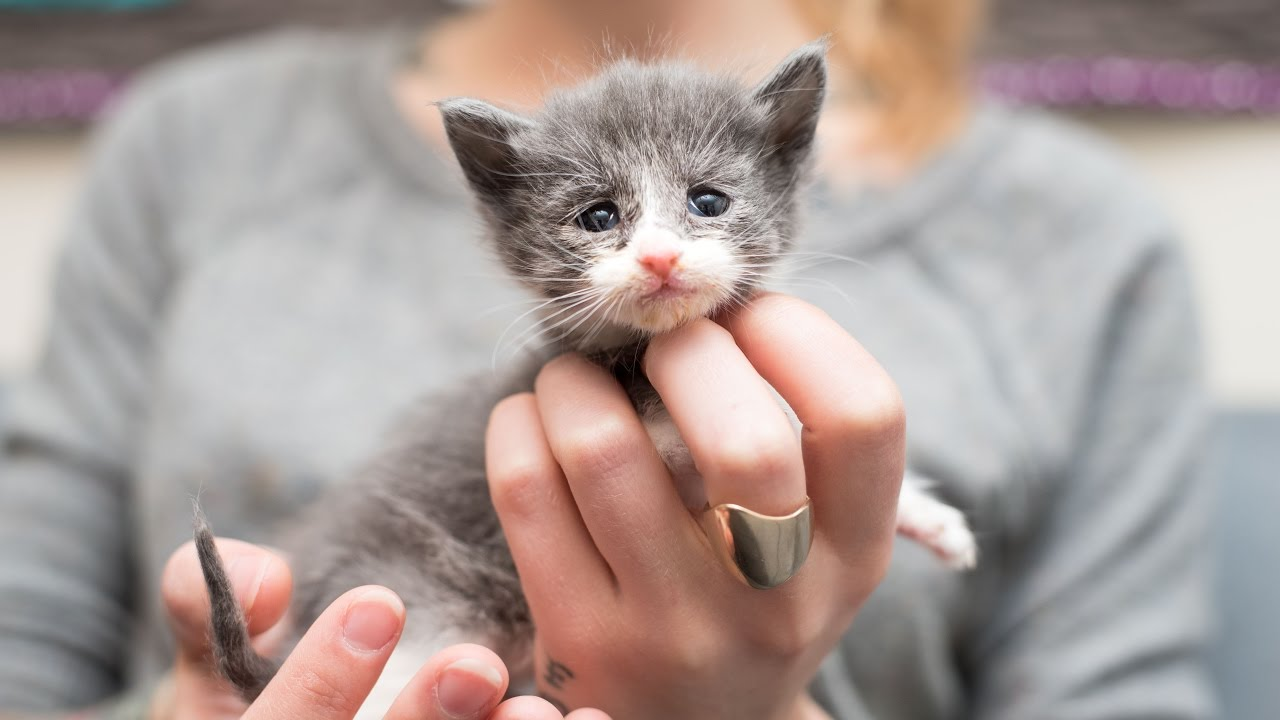
\includegraphics[width=0.5\textwidth]{Pictures/kitten-placeholder.jpg}
\caption{Scenario 3. Wavelength equal four minimum edge lengths}
\label{scen3}
\end{figure}

\textbf{Scenario 4:} wavelength is larger than 4 minimum cell edge lengths. In this condition, the pressure fluctuation performs one cycle within multiple cells in the direction of the fluctuation propagation (Fig. \ref{scen4}). FVM method computes pressure from the sound wave propagation across multiple cells.

\begin{figure}[h!]
\centering % bo \centering nie wstawia dodatkowego odstępu
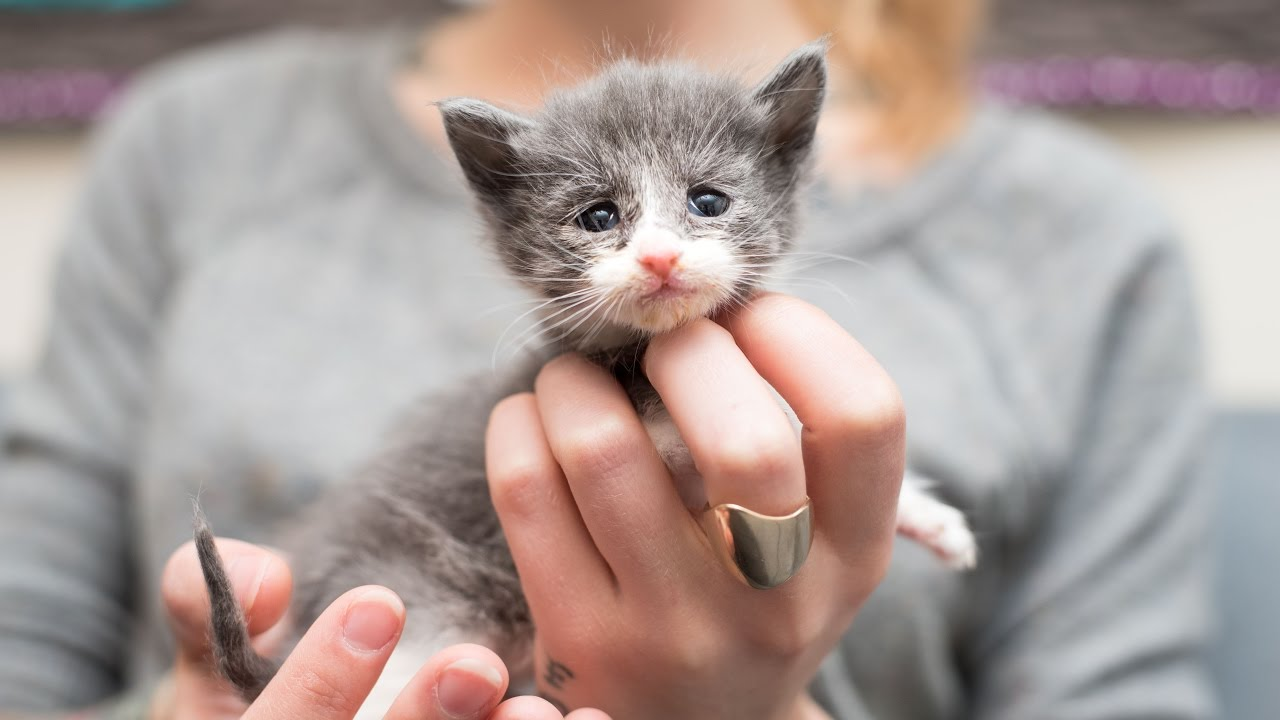
\includegraphics[width=0.5\textwidth]{Pictures/kitten-placeholder.jpg}
\caption{Scenario 4. Wavelength larger than four minimum edge lengths}
\label{scen4}
\end{figure}
%\end{itemize}

Based on these possibilities, the edge sizing of the finite volume cell should be at least four times smaller than the shortest wavelength expected in the flow field.

As there is no information on the pressure fluctuations in the flow field, the range of the further analyses will be limited to audible range of 20Hz to 20 000Hz. The wavelengths are calculated by formula \ref{eq:wl} and divided by four to obtain the required cell sizing. The velocity of sound obtained by equation \ref{eq:sos} with reference temperature $T = 300K$. The results for outermost sound frequencies of the audible range are presented in table \ref{tab:meshsize}

\begin{table}[htb!]
\centering
\caption{Test case boundary conditions} \label{tab:meshsize}
\begin{tabular}{ | r | l | l | } \hline
Frequency [Hz] & Wave length [m] & Cell size [m] \\ \hline \hline
20 & 17.390 & 4.347  \\ \hline
20 000 & 0.01739 & 0.004347 \\ \hline
\end{tabular}
\end{table}

%----------------------------------------------------------------------------------------
%	SECTION
%----------------------------------------------------------------------------------------
\section{Timestep requirements} \label{timestepsize}
There are two limiting factors for timestep requirements. The high frequency signal is limited by the timestep size, whereas the low frequencies are limited to the total number of timesteps and physical flow time calculated. The timestep size is calculated first.

Once sizing of the mesh is established, time at which the fluctuation passes the cell is established by simple formula \ref{eq:vel2}. Distance $s$ is the cell edge sizing, obtained as in section \ref{meshsize} and the relation between cell size and wave length is presented in equation \ref{eq:dist}.

\begin{equation} \label{eq:vel2}
a = \frac{s}{t}
\end{equation}

Where

\begin{equation} \label{eq:time}
t = \frac{1}{f}
\end{equation}

\begin{equation} \label{eq:dist}
s = \frac{\lambda}{4}
\end{equation}

By rearranging the equation \ref{eq:vel2} to solve for $t$ and substituting $\lambda$ by \ref{eq:wl} we obtain:

\begin{equation} \label{eq:mintime}
t = \frac{s}{a} = \frac{\lambda}{4a} = \frac{a}{f} \cdot \frac{1}{4a} = \frac{1}{4f}
\end{equation}

Equation \ref{eq:mintime} shows that time step for the analysis is dependent from the expected value of high frequency fluctuations. Four scenarios can be discussed.

\textbf{Scenario 1:} timestep is smaller than 1/4 of the fluctuation period (Fig. \ref{time1}).

\begin{figure}[h!]
\centering % bo \centering nie wstawia dodatkowego odstępu
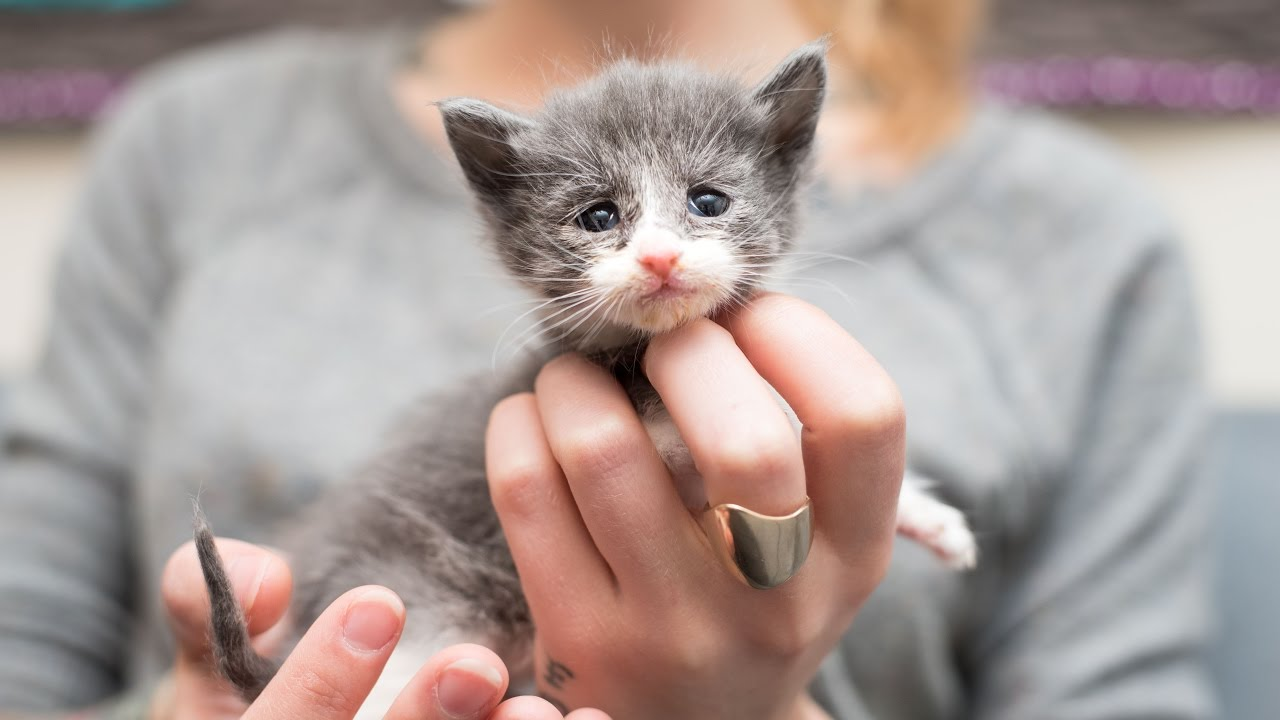
\includegraphics[width=0.5\textwidth]{Pictures/kitten-placeholder.jpg}
\caption{Scenario 1. Timestep smaller than 1/4 of fluctuation period}
\label{time1}
\end{figure}

\textbf{Scenario 2:} timestep is equal to the  1/4 of the fluctuation period (Fig. \ref{time2}).

\begin{figure}[h!]
\centering % bo \centering nie wstawia dodatkowego odstępu
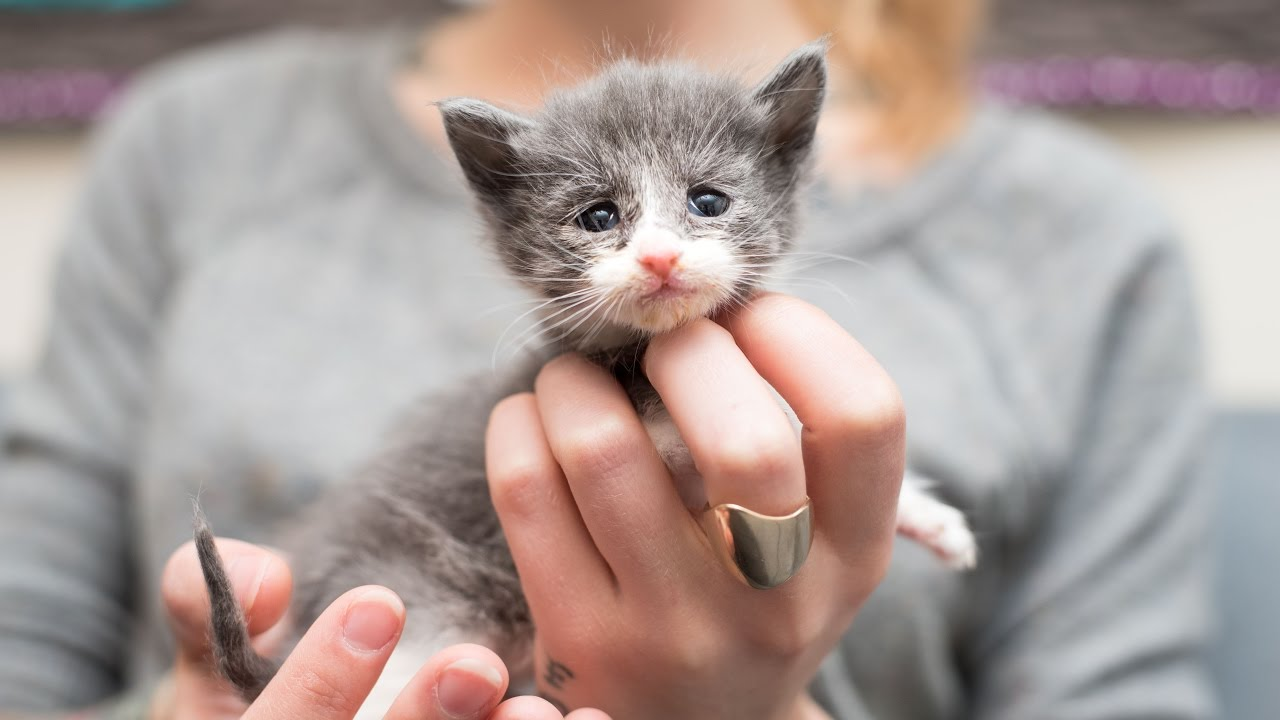
\includegraphics[width=0.5\textwidth]{Pictures/kitten-placeholder.jpg}
\caption{Scenario 2. Timestep equal to 1/4 of fluctuation period}
\label{time2}
\end{figure}

\textbf{Scenario 3:} timestep is equal to fluctuation period (Fig. \ref{time3}).

\begin{figure}[h!]
\centering % bo \centering nie wstawia dodatkowego odstępu
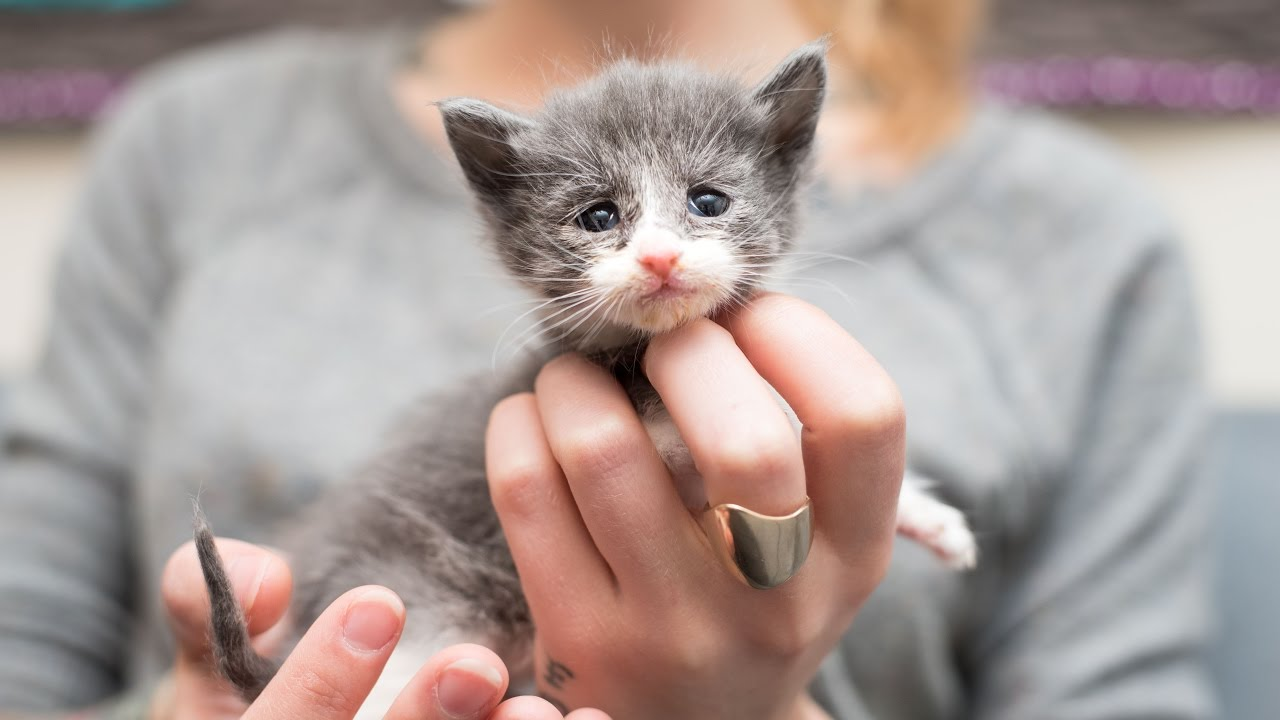
\includegraphics[width=0.5\textwidth]{Pictures/kitten-placeholder.jpg}
\caption{Scenario 3. Timestep equal to fluctuation period}
\label{time3}
\end{figure}

\textbf{Scenario 4:} timestep is larger that fluctuation period (Fig. \ref{time4}).

\begin{figure}[h!]
\centering % bo \centering nie wstawia dodatkowego odstępu
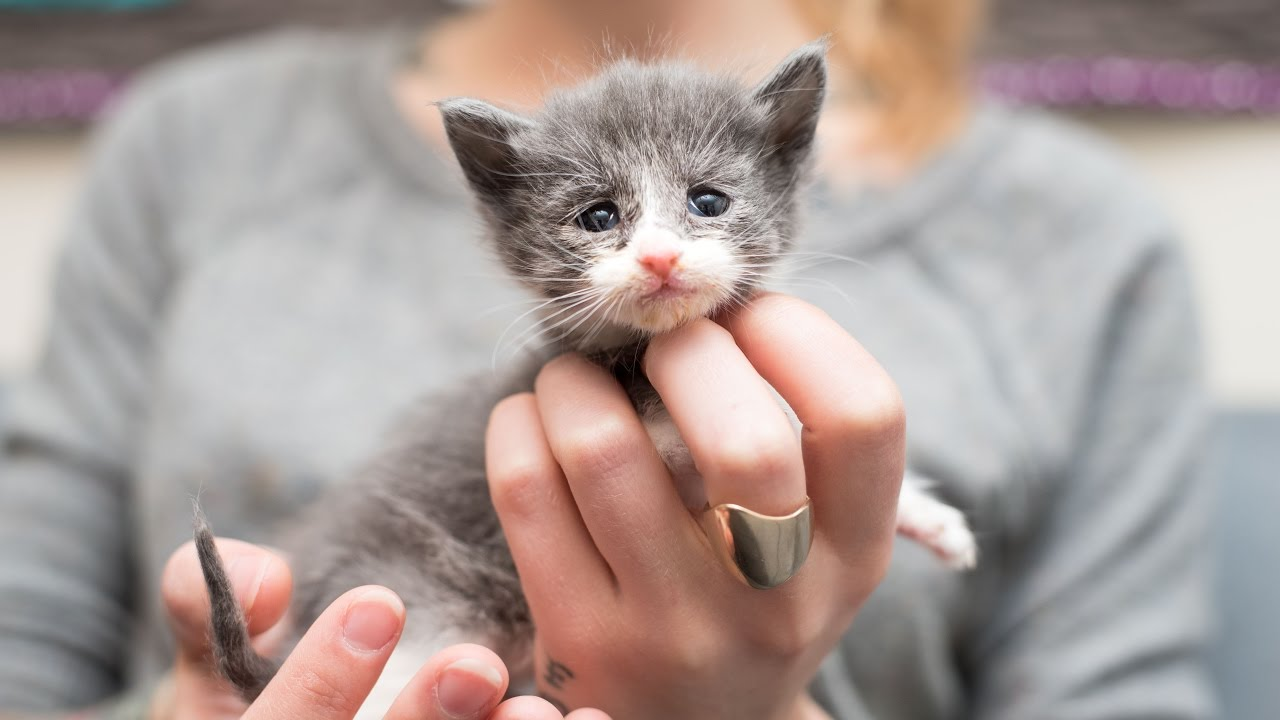
\includegraphics[width=0.5\textwidth]{Pictures/kitten-placeholder.jpg}
\caption{Scenario 4. Timestep is larger than fluctuation period}
\label{time4}
\end{figure}
%\end{itemize}

In order to capture frequencies on the low end of the spectrum, the analysis must be performed long enough to capture at least a single, with optimum 5 or more periods, of the desired low frequency. Assuming lower end of the audible frequency spectrum, the 20Hz frequency, the simulation time must resemble at least 0.05s of flow time with optimum 0.25s of flow time at given timestep.


%----------------------------------------------------------------------------------------
%	SECTION
%----------------------------------------------------------------------------------------
\section{Limiting factors of the direct approach} \label{limits}
Provided approach is solely a post processing approach relying on data provided by a CFD analysis. In order to obtain reasonable results down the process, the analysis itself mus be capable of delivering pressure fluctuations that can be considered as acoustic in source. 

Utilizing a numerical model that averages flow field in terms of numerical methods, treatment of turbulent motions or mesh of insufficient quality, will return a pressure flow field that all acoustic kind fluctuations filtered out. 

Pressure signal used by this approach is given by a list of real scalar values for each node or cell centroid for each timestep. Therefore obtaining phase shift of the ordinary sinuses components of pressure signal may be challenging, if at all possible, and relies solely on further postprocessing of generated data. 

The range of frequencies captured by this method depends on the mesh sizing and timestep sizing. Therefore, if the range of expected frequencies is known or at least estimated, the mesh sizing and timestep size can be adjusted for the given case.
 
Direct formulation acoustic analysis requires storing pressure and velocity information from all timesteps and then performing averaging over all timesteps. For analysis within audible range 4000 timesteps is required for one 20Hz period. Considering the mesh sizing requirements, the mesh cell count will rise up to tens of millions, which makes storing and managing the data somewhat difficult. Averaging the timestep data, obtaining sound pressure levels, sound intensity levels and respective decibel levels. 

For incompressible flows or flows with low pressure gradients or without shock waves such approach is exaggerated. Should the flow occur in majority in ambient conditions (i.e. low velocity jet in free stream), the offset from the ambient pressure may be computed "on-the-fly".

Although computationally expensive, such approach is required in flows with very high pressure gradients, as it is impossible to establish one reference pressure for whole flow field.

%Morbi rutrum odio eget arcu adipiscing sodales. Aenean et purus a est pulvinar pellentesque. Cras in elit neque, quis varius elit. Phasellus fringilla, nibh eu tempus venenatis, dolor elit posuere quam, quis adipiscing urna leo nec orci. Sed nec nulla auctor odio aliquet consequat. Ut nec nulla in ante ullamcorper aliquam at sed dolor. Phasellus fermentum magna in augue gravida cursus. Cras sed pretium lorem. Pellentesque eget ornare odio. Proin accumsan, massa viverra cursus pharetra, ipsum nisi lobortis velit, a malesuada dolor lorem eu neque.



%----------------------------------------------------------------------------------------
%	SECTION
%----------------------------------------------------------------------------------------
%\section{Basic conservation equations in CFD}
%-----------------------------------
%	SUBSECTION
%-----------------------------------
%\subsection{Momentum equations}
%Nunc posuere quam at lectus tristique eu ultrices augue venenatis. Vestibulum ante ipsum primis in faucibus orci luctus et ultrices posuere cubilia Curae; Aliquam erat volutpat. Vivamus sodales tortor eget quam adipiscing in vulputate ante ullamcorper. Sed eros ante, lacinia et sollicitudin et, aliquam sit amet augue. In hac habitasse platea dictumst.

%-----------------------------------
%	SUBSECTION
%-----------------------------------
%\subsection{Continuity Equations}
%Morbi rutrum odio eget arcu adipiscing sodales. Aenean et purus a est pulvinar pellentesque. Cras in elit neque, quis varius elit. Phasellus fringilla, nibh eu tempus venenatis, dolor elit posuere quam, quis adipiscing urna leo nec orci. Sed nec nulla auctor odio aliquet consequat. Ut nec nulla in ante ullamcorper aliquam at sed dolor. Phasellus fermentum magna in augue gravida cursus. Cras sed pretium lorem. Pellentesque eget ornare odio. Proin accumsan, massa viverra cursus pharetra, ipsum nisi lobortis velit, a malesuada dolor lorem eu neque.

%\subsection{Energy equation}
%Morbi rutrum odio eget arcu adipiscing sodales. Aenean et purus a est pulvinar pellentesque. Cras in elit neque, quis varius elit. Phasellus fringilla, nibh eu tempus venenatis, dolor elit posuere quam, quis adipiscing urna leo nec orci. Sed nec nulla auctor odio aliquet consequat. Ut nec nulla in ante ullamcorper aliquam at sed dolor. Phasellus fermentum magna in augue gravida cursus. Cras sed pretium lorem. Pellentesque eget ornare odio. Proin accumsan, massa viverra cursus pharetra, ipsum nisi lobortis velit, a malesuada dolor lorem eu neque.

%----------------------------------------------------------------------------------------
%	SECTION 2
%----------------------------------------------------------------------------------------
%\section{Resolving turbulence}

%-----------------------------------
%	SUBSECTION
%-----------------------------------
%\subsection{RANS formulation of turbulent flow}
%Morbi rutrum odio eget arcu adipiscing sodales. Aenean et purus a est pulvinar pellentesque. Cras in elit neque, quis varius elit. Phasellus fringilla, nibh eu tempus venenatis, dolor elit posuere quam, quis adipiscing urna leo nec orci. Sed nec nulla auctor odio aliquet consequat. Ut nec nulla in ante ullamcorper aliquam at sed dolor. Phasellus fermentum magna in augue gravida cursus. Cras sed pretium lorem. Pellentesque eget ornare odio. Proin accumsan, massa viverra cursus pharetra, ipsum nisi lobortis velit, a malesuada dolor lorem eu neque.

%-----------------------------------
%	SUBSECTION
%-----------------------------------
%\subsection{DDES Formulation of turbulence}
%Morbi rutrum odio eget arcu adipiscing sodales. Aenean et purus a est pulvinar pellentesque. Cras in elit neque, quis varius elit. Phasellus fringilla, nibh eu tempus venenatis, dolor elit posuere quam, quis adipiscing urna leo nec orci. Sed nec nulla auctor odio aliquet consequat. Ut nec nulla in ante ullamcorper aliquam at sed dolor. Phasellus fermentum magna in augue gravida cursus. Cras sed pretium lorem. Pellentesque eget ornare odio. Proin accumsan, massa viverra cursus pharetra, ipsum nisi lobortis velit, a malesuada dolor lorem eu neque.

%-----------------------------------
%	SUBSECTION
%-----------------------------------
%\subsection{DDES Formulation of turbulence}
%Morbi rutrum odio eget arcu adipiscing sodales. Aenean et purus a est pulvinar pellentesque. Cras in elit neque, quis varius elit. Phasellus fringilla, nibh eu tempus venenatis, dolor elit posuere quam, quis adipiscing urna leo nec orci. Sed nec nulla auctor odio aliquet consequat. Ut nec nulla in ante ullamcorper aliquam at sed dolor. Phasellus fermentum magna in augue gravida cursus. Cras sed pretium lorem. Pellentesque eget ornare odio. Proin accumsan, massa viverra cursus pharetra, ipsum nisi lobortis velit, a malesuada dolor lorem eu neque.